\documentclass{article}
\usepackage[utf8]{inputenc}
\usepackage[T1]{fontenc}
\usepackage[utf8]{inputenc}
\usepackage{lmodern}
\usepackage[a4paper, margin=1in]{geometry}
\usepackage{graphicx} 
\renewcommand{\thesubsection}{\alph{subsection}}

\usepackage{minted}
\large
\title{CS 520}
\begin{document}
\begin{titlepage}
	\begin{center}
    \line(1,0){300}\\
    [0.65cm]
	\huge{\bfseries Assignment 1}\\
	\line(1,0){300}\\
	\textsc{\Large CS 520: INTRODUCTION TO ARTIFICIAL INTELLIGENCE \\ Fast Trajectory Replanning}\\
	\textsc{\LARGE \today}\\
	[5.5cm]     
	\end{center}
	\begin{flushright}
		\textsc{\Large Satyabrat Bhol\\sb2311}\\
		[0.5cm]
		\textsc{\Large Pranoy Sarath\\ps1279}\\
		[0.5cm]
            \textsc{\Large Pradeep Roy Yadlapalli\\py160}\\
		[0.5cm]
	\end{flushright}
\end{titlepage}


\section*{Part 0 - Setup your Environments}

\begin{flushleft}
We have written custom code to generate the mazes. It takes in the dimensions of the environment, along with the number of grid environments to be generated. This follows a Depth First Search approach and for each of the cells, we randomly generate a number within the range() and if the random number falls within the range(), we assume it to be a blocked cell. \\
Once the blocked cells are generated for all the environments, the list would be returned. \\
As for the project experiment, we will be fixing the size of the environment to 101 X 101 and 50 such environments will be created.
\end{flushleft}
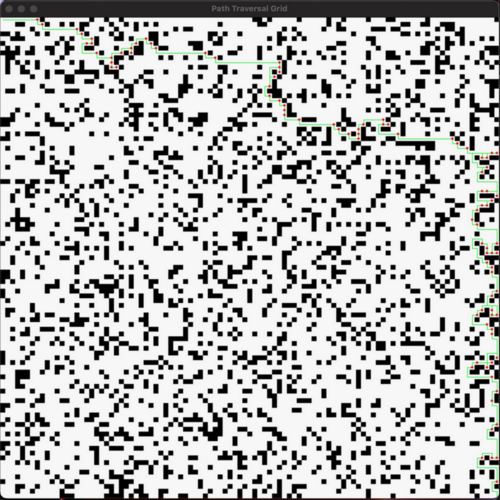
\includegraphics{grid.png}
\section*{Part 1 - Understanding the methods}
\begin{enumerate}
\item 
\begin{flushleft}
The function that is used to evaluate the cost is f(n) = g(n) + h(n) where g(n) is the distance traveled by the robot from the start state and h(n) is the heuristic function value for the given cell and the target. For the maze, we are using Manhattan distance as the heuristic. \\
The following observations have been made with reference to Fig 8. on the Assignment \\
For the cell E3,  g(n) = 1 and h(n) = 2 => f(n) = 3 \\
For the cell D2, g(n) = 1 and h(n) = 4  => f(n) = 5 \\
Since the overall cost f(n) is lower for D2 on comparing with E3, the robot first visits D2 and expands all its neighbors, and adds them to the open list
\end{flushleft}
\item
\begin{flushleft}
The A star algorithm is an optimized version of a basic DFS. \\
In DFS, each node has the same cost to reach the goal, and as per the algorithm, if a path exists from the source to the goal, it would eventually reach the target though we cannot ensure that it will be the optimal path. The worst-case time complexity for this is O( |V| + |E|) where V represents the number of vertices and E represents the number of edges. Thus for our environment of size 101 x 101 , we are bound to reach the target in $O(5x10^5)$ which would be the finite upper bound.
\end{flushleft}
\end{enumerate}
\newpage

\section*{Part 2 - The Effects of Ties}
\begin{flushleft}
We observed that using higher g-cost for breaking ties resulted in a lower number of overall expanded nodes which led to better running time. \\
Higher g-cost seems to run $18\%$ faster than lower g-cost nodes. \\
The idea here is that, if we go for lower g-cost  nodes, then we will be expanding nodes that are farther away from the goal. Thus expanding the nodes which are closer to the goal (that is those having higher g-cost) resulted in better performance/run-time.
\end{flushleft}

\section*{Part 3 - Forward vs. Backward}
\begin{flushleft}
The running time comparison between Repeated Forward A star and the Repeated Backward A star was quite similar. For certain cases, we found the Backward A star performing better, while for other cases it was the Forward A star.\\ Performance comparison was based on the run-time as well as the number of expanded cells.
\end{flushleft}


\section*{Part 4 - Heuristics in the Adaptive $A^*$}
\begin{enumerate}
\item 
\begin{flushleft}
The agent can only move in four directions i.e right, left, up and down, which is the criteria of Manhattan distance. So the shortest path from the source to the destination will be the Manhattan distance given the agent is not allowed to move diagonally. Therefore the Manhattan distances are consistent.\\
If in case diagonal movement is allowed, then the distances heuristics will be overestimated. (Might have to opt for Euclidean distances in such cases).
\end{flushleft}
\item
\begin{flushleft}
A heuristic is consistent if the heuristic step cost never overestimates the actual step cost. \\
Let the step cost of going from $n$ to $n'$ be $c(n,a,n')$, the original step cost be $c$ and the final step cost be $c'$. Then, $h(n) <= c(n,a,n')+h(n')$. \\ The updated heuristic will $h_up(n) <= c(n,a,n')+h_up(n')$ which is lesser than $c'(n,a,n')$. \\ Thus proves the consistency.
\end{flushleft}
\end{enumerate}

\section*{Part 5 - Heuristics in the Adaptive $A^*$}
\begin{flushleft}
We observed that the number of expanded nodes for the adaptive A star is always less than or equal to that of the A star algorithm, as a result, the adaptive A star algorithm performance was either approximately equal to or better than the Repeated forward A star algorithm.
\end{flushleft}
\newpage

\section*{Part 6 - Statistical Significance}
\begin{flushleft}
Statistical Interpretation of the above search algorithms by analyzing a few basic values like mean, median might give a possible insight. \\
Let say for mean - mean (algo 1) > mean(algo 2), but the Mean run-time of algo 1 is $4\%$
run time of algo 2 then we can say that the run time distributions of the algorithms are not significantly different from each other and the mean difference is mainly due to noise. \\
Similarly, for median - median (algo 1) > median(algo 2) but the median run time of algo 1 is $11\%$ faster than
the median run time of algo 2 then we can say that the run time distributions of the algorithms are significantly different from each other and it is systematic in nature. \\
Since the above two interpretations do not offer much credibility to statistical hypothesis testing
methods we could use a Two-sample T-test. \\
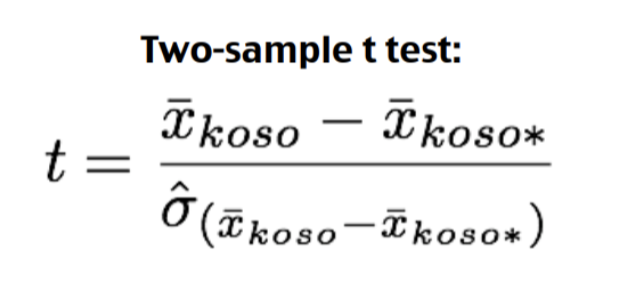
\includegraphics{test.png}
\end{flushleft}


\end{document}











